\documentclass{beamer}

\author{Yu Cong}
\title[Minimizing sum of pwl convex function]{Minimizing the Sum of Piecewise Linear Convex Functions}
\date{\today}

% \AtBeginSection[]{
%     \frame{\frametitle{Outline}\tableofcontents[currentsection, 
%     subsectionstyle=show/show/shaded]}
% }
    
% Copyright 2018 by Zhibo Wang
%
% This file may be distributed and/or modified
% under the LaTeX Project Public License


\definecolor{beamer@simple@color}{RGB}{12 72 66} % bluegreen
\DeclareOptionBeamer{gray}{\definecolor{beamer@simple@color}{gray}{#1}}
\DeclareOptionBeamer{rgb}{\definecolor{beamer@simple@color}{rgb}{#1}}
\DeclareOptionBeamer{RGB}[{12 72 0}]{\definecolor{beamer@simple@color}{RGB}{#1}}
\DeclareOptionBeamer{HTML}{\definecolor{beamer@simple@color}{HTML}{#1}}
\DeclareOptionBeamer{cmyk}{\definecolor{beamer@simple@color}{cmyk}{#1}}
\DeclareOptionBeamer{cmy}{\definecolor{beamer@simple@color}{cmy}{#1}}
\DeclareOptionBeamer{named}{\definecolor{beamer@simple@color}{named}{#1}}
\DeclareOptionBeamer{hsb}{\definecolor{beamer@simple@color}{hsb}{#1}}
\ProcessOptionsBeamer

% footline
% delete navigation below
\setbeamertemplate{navigation symbols}{}
% define footline
% \makeatother
\setbeamertemplate{footline}
{
  \leavevmode%
  \hbox{%
    \begin{beamercolorbox}[wd=.38\paperwidth,ht=2.25ex,dp=1ex,center]{author in head/foot}%
        \usebeamerfont{author in head/foot}\insertshortauthor
    \end{beamercolorbox}

    \begin{beamercolorbox}[wd=.62\paperwidth,ht=2.25ex,dp=1ex,center]{title in head/foot}%
        \usebeamerfont{title in head/foot}\insertshorttitle
    \end{beamercolorbox}

    % \begin{beamercolorbox}[wd=.1\paperwidth,ht=2.25ex,dp=1ex,center]{title in head/foot}%
    %     \usebeamerfont{title in head/foot}\insertframenumber{} / \inserttotalframenumber\hspace*{0ex}
    % \end{beamercolorbox}
  }

  \vskip0pt%
}
\useoutertheme{tree}
\makeatletter
\setbeamertemplate{headline}
{%
    \begin{beamercolorbox}[wd=\paperwidth,colsep=1.5pt]{upper separation line head}
    \end{beamercolorbox}
    \begin{beamercolorbox}[wd=\paperwidth,ht=2.5ex,dp=1.125ex,%
      leftskip=.3cm,rightskip=.3cm plus1fil]{title in head/foot}
      \usebeamerfont{title in head/foot}\insertshorttitle
      \usebeamerfont{section in head/foot}%
      \ifbeamer@tree@showhooks
        \setbox\beamer@tempbox=\hbox{\insertsectionhead}%
        \ifdim\wd\beamer@tempbox>1pt%
          \hskip2pt\raise1.9pt\hbox{\vrule width 5pt height0.4pt}%
          \hskip1pt%
        \fi%
      \else%  
        \hskip6pt%
      \fi%
      \insertsectionhead
      \usebeamerfont{subsection in head/foot}%
      \ifbeamer@tree@showhooks
        \setbox\beamer@tempbox=\hbox{\insertsubsectionhead}%
        \ifdim\wd\beamer@tempbox>1pt%
          \hskip2pt\raise1.9pt\hbox{\vrule width 5pt height0.4pt}%
          \hskip1pt%
        \fi%
      \else%  
        \hskip12pt%
      \fi%
      \insertsubsectionhead\hfill\insertframenumber/\inserttotalframenumber\hspace{0.5em}
    \end{beamercolorbox}
    \begin{beamercolorbox}[wd=\paperwidth,colsep=1.5pt]{lower separation line head}
    \end{beamercolorbox}
}
\makeatother
% \makeatletter
% footline color
\setbeamercolor{author in head/foot}{fg=black, bg=mygrey!5!white}
\setbeamercolor{title in head/foot}{fg=black, bg=mygrey!5!white}

% item settings
\setbeamertemplate{itemize item}{$\color{beamer@simple@color}\bullet$}
\setbeamertemplate{itemize subitem}{$\color{beamer@simple@color}\bullet$}
\setbeamertemplate{enumerate items}[square]
\setbeamertemplate{section in toc}[sections numbered]
\setbeamertemplate{subsection in toc}[square]



% color definition
\definecolor{mygrey}{rgb}{0.52, 0.52, 0.51}

\setbeamercolor{structure}{fg=beamer@simple@color, bg=mygrey!10!white}
\setbeamercolor{frametitle}{fg=beamer@simple@color, bg=white}
\setbeamercolor{block title}{bg=mygrey!14!white}
\setbeamercolor{block body}{fg=black,bg=mygrey!10!white}
\setbeamercolor{block body alerted}{bg=white}
\setbeamercolor{block title alerted}{fg=beamer@simple@color,bg=white}
\setbeamercolor{alerted text}{fg=beamer@simple@color}
\setbeamerfont{block title alerted}{series=\mdseries}
\setbeamerfont{alerted text}{series=\bfseries\boldmath}
\hypersetup{colorlinks,linkcolor=,urlcolor=beamer@simple@color!80!white}
\usefonttheme[onlymath]{serif}
\setbeamerfont{frametitle}{series=\bfseries\boldmath}
\setbeamerfont{block title}{series=\bfseries\boldmath}
\setbeamerfont{title}{series=\bfseries\boldmath}
\setbeamertemplate{frametitle}{\insertframetitle\par\vskip-8pt\hrulefill} % add line under frametitle

% % metropolis
% % \definecolor{beamer@simple@color}{RGB}{35 54 58}
% % no outer theme
% \setbeamerfont{frametitle}{series=\bfseries}
% \setbeamercolor{frametitle}{fg=white, bg=beamer@simple@color}
% \setbeamerfont{block title}{series=\bfseries}
% \setbeamerfont{block title alerted}{series=\bfseries}
% \definecolor{alertcol}{RGB}{232 133 52}
% \setbeamercolor{block title alerted}{fg=alertcol,bg=white}
% \setbeamerfont{alerted text}{series=\mdseries}
% \setbeamercolor{alerted text}{fg=alertcol}
\setbeamercolor{block title}{bg=mygrey!25!white}
\setbeamercolor{block body}{fg=black,bg=mygrey!13!white}



% ----------------------------------------------------------------------
%  Simple math stuff
% ----------------------------------------------------------------------
\renewcommand{\subset}{\subseteq}
% ---- SYMBOLS ----
\let\e\varepsilon               % a ``real'' epsilon — better yet, just use Unicode ε.
%
%  I give up.  These are in the wrong font, but my kludged versions 
%  LOOK like kludges, especially \Z, \Q, and \C.
%
\def\Real{\mathbb{R}}
\def\Proj{\mathbb{P}}
\def\Hyper{\mathbb{H}}
\def\Integer{\mathbb{Z}}
\def\Natural{\mathbb{N}}
\def\Complex{\mathbb{C}}
\def\Rational{\mathbb{Q}}

\let\N\Natural
\let\Q\Rational
\let\R\Real
\let\Z\Integer
\def\Rd{\Real^d}
\def\RP{\Real\Proj}
\def\CP{\Complex\Proj}



% ---- OPERATORS (requires amsmath) ----
\def\aff{\operatorname{aff}}        
\def\area{\operatorname{area}}
\def\argmax{\operatornamewithlimits{arg\,max}}
\def\argmin{\operatornamewithlimits{arg\,min}}
\def\Aut{\operatorname{Aut}}        % Automorphism group
\def\card{\operatorname{card}}  % cardinality, deprecated for \abs
\def\conv{\operatorname{conv}}  
\def\E{\operatorname{E}}            % Expectation: $\E[X]$ (like \Pr)
\def\EE{\operatornamewithlimits{E}}
\def\Hom{\operatorname{Hom}}        % Homomorphism group
\def\id{\operatorname{id}}      % identity
\def\im{\operatorname{im}}      % image
\def\lcm{\operatorname{lcm}}
\def\lfs{\operatorname{lfs}}        % local feature size
\def\poly{\operatorname{poly}}
\def\polylog{\operatorname{polylog}}
\def\rank{\operatorname{rank}}
\def\rel{\operatorname{rel\,}}  % relative (interior, boundary, etc.)
\def\sgn{\operatorname{sgn}}
\def\vol{\operatorname{vol}}        % volume

\def\fp#1{^{\underline{#1}}}        % falling powers: $n\fp{d}$
\def\rp#1{^{\overline{#1}}}     % rising powers:  $n\rp{d}$

\def\setsymdiff{\operatorname{\triangle}}
% % --- Darts and fences ---
% % less nice replacements for stmaryrd characters
% \@ifundefined{shortrightarrow}{\let\shortrightarrow\rightarrow}{}
% \@ifundefined{shortleftarrow}{\let\shortleftarrow\leftarrow}{}
% \@ifundefined{shortuparrow}{\let\shortuparrow\uparrow}{}
% \@ifundefined{shortdownarrow}{\let\shortdownarrow\downarrow}{}

\def\arcto{\mathord\shortrightarrow}
\def\arcfrom{\mathord\shortleftarrow}
\def\arc#1#2{#1\arcto#2}
\def\cra#1#2{#1\mathord\shortleftarrow#2}
\def\fence#1#2{#1\mathord\shortuparrow#2}
\def\ecnef#1#2{#1\mathord\shortdownarrow#2}

% --- Cheap displaystyle operators ---
\def\Frac#1#2{{\displaystyle\frac{#1}{#2}}}
\def\Sum{\sum\limits}
\def\Prod{\prod\limits}
\def\Union{\bigcup\limits}
\def\Inter{\bigcap\limits}
\def\Lor{\bigvee\limits}
\def\Land{\bigwedge\limits}
\def\Lim{\lim\limits}
\def\Max{\max\limits}
\def\Min{\min\limits}

% ---- RELATORS ----
\def\deq{\stackrel{\scriptscriptstyle\triangle}{=}} % Use := instead.
\def\into{\DOTSB\hookrightarrow}        % = one-to-one
\def\onto{\DOTSB\twoheadrightarrow}
\def\inonto{\DOTSB\lhook\joinrel\twoheadrightarrow}
\def\from{\leftarrow}
\def\tofrom{\leftrightarrow}
\def\mapsfrom{\mathrel{\reflectbox{$\mapsto$}}}
\def\longmapsfrom{\mathrel{\reflectbox{$\longmapsto$}}}

% ---- DELIMITER PAIRS ----
% --- always self-scaling delmiter pairs ---
\def\set#1{\left\{ #1 \right\}}
\def\floor#1{\left\lfloor #1 \right\rfloor}
\def\ceil#1{\left\lceil #1 \right\rceil}
\def\seq#1{\left\langle #1 \right\rangle}
\def\abs#1{\left| #1 \right|}
\def\norm#1{\left\| #1 \right\|}
\def\paren#1{\left( #1 \right)}     % need better macro name!
\def\brack#1{\left[ #1 \right]}     % need better macro name!
\def\indic#1{\left[ #1 \right]}     % indicator variable; Iverson notation


% \useoutertheme{tree}
    
\begin{document}
\begin{frame}[plain]
    % Print the title page as the first slide
    \titlepage
\end{frame}

\begin{frame}[plain]{Plan}
    \tableofcontents
\end{frame}

\section{Problems \& Definitions}
\begin{frame}{$\min \sum f_i(a_i\cdot x-b_i)$}
\begin{problem}
    Given $n$ piecewise linear convex functions $f_1,...,f_n:\R \to \R$ of total $m$ breakpoints, and $n$ linear functions $a_i\cdot x-b_i:\R^d\to \R$, find $\min_x \sum_i f_i(a_i\cdot x-b_i)$.
\end{problem}
\begin{figure}
    \centering
    \begin{subfigure}{.5\textwidth}
      \centering
      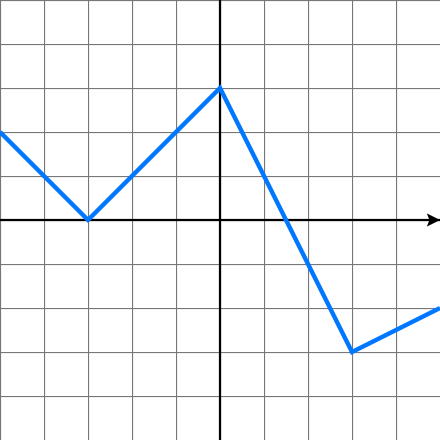
\includegraphics[width=.4\linewidth]{images/Piecewise_linear_function.svg.png}
      \caption{A 1D pwl function with 4 line segments and 3 breakpoints}
      \label{fig:sub1}
    \end{subfigure}%
    \begin{subfigure}{.5\textwidth}
      \centering
      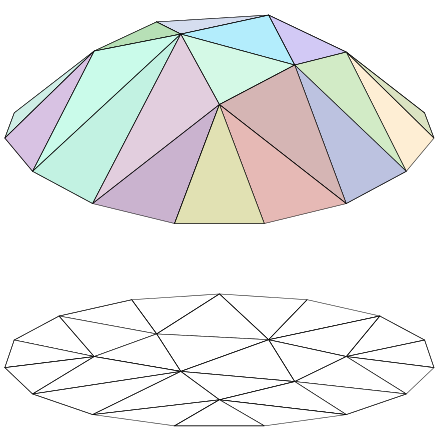
\includegraphics[width=.4\linewidth]{images/Piecewise_linear_function2D.png}
      \caption{A 2D pwl concave function}
      \label{fig:sub2}
    \end{subfigure}
    % \caption{A figure with two subfigures}
    \label{fig:1}
    \end{figure}
    $f_i(a_i\cdot x-b_i):\R^d\to \R$ is also piecewise linear convex.
\end{frame}

\begin{frame}{General piecewise linear convex function in $\R^d$}
\begin{definition}[piecewise linear convex function in $\R^d$]\label{def:pwlc}
\[
g(x)=\max \{a_1^Tx+b_1,\ldots,a_L^Tx+b_L\}
\]
\end{definition}

Every piecewise linear convex function in $\R^d$ can be expressed in this form.\footnote{S.P. Boyd, L. Vandenberghe, \textbf{Convex optimization}, Cambridge University Press, Cambridge, UK ; New York, 2004.}

However, observe that in our problem the piecewise linear convex function is not that general. It is a composition of a linear mapping and an 1D piecewise linear convex function.

\end{frame}

\begin{frame}{$f\circ l\not \equiv g$}
    \begin{proof}
    \small
    Consider a piecewise linear convex function $g:\R^2\to \R$. $g$ can be viewed as the maximum of a set of planes in $\R^3$.

    Consider a series of points $P=\set{p_1,p_2,...,p_k}$ on the 2D plane. After applying the linear mapping to $P$, we will get a sequence of numbers(points in 1D) $P'=\set{p_1',p_2',...,p_k'}$. We assume that $P'$ is non-decreasing. Note that the value of $g$ on $P'$ is always unimodal since $g$ is convex. However, the value of $f$ on $P$ may not be unimodal. Thus the composition of a linear mapping and a pwl convex function in 1D is not equivalent to pwl convex functions in high dimensions.
    \end{proof}
\end{frame}

\section{Properties}
\begin{frame}[allowframebreaks]{A linear time algorithm}
    \begin{problem}
        Given $n$ piecewise linear convex functions $f_1,...,f_n:\R \to \R$ of total $m$ breakpoints, and $n$ linear functions $a_i\cdot x-b_i:\R^d\to \R$, find $\min_x \sum_i f_i(a_i\cdot x-b_i)$.
    \end{problem}
    This can be solve in $O(2^{2^d} (m+n))$ through Megiddo's Low dimension LP algorithm.\footnote{Nimrod Megiddo. Linear programming in linear time when the dimension is fixed. J. ACM, 31(1):114–127, jan 1984.}

    Let $n_i$ be the number of line segments in $f_i$. Note that $\sum_i n_i=m+n$.

    We can formulate the optimization problem as the following linear program,
    \newpage

    \begin{align*}
        \min &\sum_{i=1}^n f_i\\
        s.t. \quad f_i&\geq \alpha_j(a_i\cdot x -b_i)-\beta_j \quad \forall i\in[n], \forall j\\
    \end{align*}

    where $\alpha_j x - \beta_j$ is the $j$'th line segment on $f_i$.

    There will be $m+n$ constraints in total.
\end{frame}

\section{LP in Low Dimensions}
\begin{frame}[allowframebreaks]{Megiddo's algorithm}%
    \mybox[oliver!20]{
        \tiny
        \url{https://people.inf.ethz.ch/gaertner/subdir/texts/own_work/chap50-fin.pdf}
    }
    The dimension $d$ (in our problem, the dimension of $x$) is small while the number of constraints are huge. We need only $d$ linearly independent tight constraints to identify the optimal solution $x^*$.
    Thus most of the constraints are useless.
    \BlankLine


    \textbf{For one constraint, how can we know where does $x^*$ locate with respect to it?}

    Through inquiries. Let $a\cdot x \leq b$ be the constraint. Define 3 hyperplanes, $a\cdot x = c$ where $c\in \set{b,b-\e,b+\e}$. Now solve three $d-1$ dimension linear programming. The largest of the three objective functions tells us where $x^*$ lies with respect to the
    hyperplane.

    \newpage
    Finding the optimal solution $x^*$ is therefore equivalent to the following problem,
    \begin{problem}[Multidimensional Search Problem]
        Suppose that there exists a point $x^*$ which is not known to us, but there is a oracle that can tell the position of $x^*$ relative to any hyperplane in $\R^d$. Given $n$ hyperplanes, we want to know the position of $x^*$ relative to each of them.
    \end{problem}

    \textbf{What about 1 dimension search?} A fastest way will be using the linear time median algorithm. We can find the median of $n$ numbers and call the oracle to compare the median with $x^*$. Thus with $O(n)$ time median finding and one oracle call, we find the relative position of $n/2$ elements relative to $x^*$.

    \newpage

    If we can do similar things in $\R^d$, i.e., there is a method which makes $A(d)$ oracle calls and determines at least $B(d)$ fraction of relative positions, then we can apply this method $\log_{\frac{1}{1-B(d)}} n$ times to find all relative positions.

    Note that in 1 dimension, $A(1)=1$ and $B(1)=1/2$ (call oracle to compare $x^*$ and the median). In $\R^d$, our oracle is the recursive inquiry.

    A trivial method will be iterating on all hyperplanes and calling the oracle on each one, since there is no \emph{median} of a set of hyperplanes in $\R^d$. The complexity recurrence is 
    \[T(n,d)=n(3T(n-1,d-1)+O(nd))\] 
    Note that in this setting $A(d)=1$ and $B(d)=1/n$.

    \newpage
    Megiddo designed a clever method where $A(d)=2^{d-1}$ and $B(d)=2^{-(2^d-1)}$.

    \begin{lemma}
        \begin{figure}
            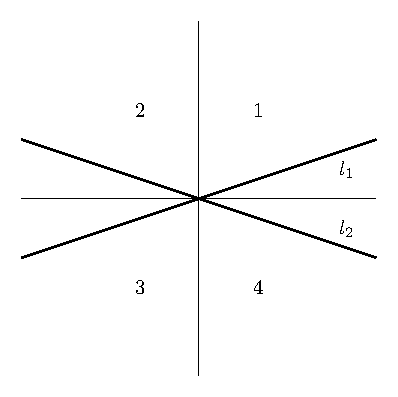
\includegraphics[width=.3\textwidth]{images/1234.pdf}
        \end{figure}
        Given two lines through the origin with slopes of opposite sign, knowing which quadrant $x^*$ lies in allows us to locate it with respect to at least one of the lines.
    \end{lemma}
    \newpage
    Let $l_H$ be the intersection of hyperplane $H$ and $x_1x_2$ plane.
    Compute a partition $S_1\sqcup S_2=\mathcal H$. 
    $H\in S_1$ iff $l_H$ has positive slope. Otherwise $l_H\in S_2$. We further assume that $|S_1|=|S_2|=n/2$.
    \noindent
    \begin{minipage}[t]{.5\textwidth}
    \begin{figure}
        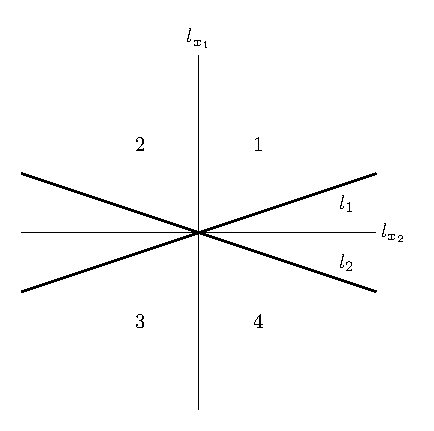
\includegraphics[width=.85\textwidth]{images/4l1234.pdf}
    \end{figure}
    \end{minipage}% <---------------- Note the use of "%"
    \begin{minipage}[t]{.5\textwidth} 
        \vspace{25pt}
        Now we have $n/2$ pairs $(H_1,H_2)$, where $H_i\in S_i$. Let $l_i$ be the intersection of $H_i$ and $x_1x_2$ plane.
        Let $H_{x_i}$ be the linear combination of $H_1$ and $H_2$ s.t. $x_i$ is eliminated.
    \end{minipage}

    { 
    % Now we have $n/2$ pairs $(H_1,H_2)$, where $H_i\in S_i$. Let $l_i$ be the intersection of $H_i$ and $x_1x_2$ plane.
    % Let $H_{x_i}$ be the linear combination of $H_1$ and $H_2$ s.t. $x_i$ is eliminated.
    By the previous lemma, calling oracle on $l_{x_1}$ and $l_{x_2}$ locate $x^*$ with respect to at least one of $H_1$ and $H_2$.}
    \newpage
    Input: $S_1,S_2$ and the pairs.
    \begin{enumerate}
        \item recursively locate $x^*$ respect to $B(d-1)n/2$ hyperplanes($H_{x_i}$) with $A(d-1)$ oracle calls in $S_1$.
        \item locate with respect to a $B(d-1)$-fraction of corresponding paired hyperplanes in $S_2$.
        \item There are still $(1-{B(d-1)}^2)/2$-fraction of hyperplanes for which we do not know the relative position with $x^*$. Run this algorithm on these hyperplanes.
    \end{enumerate}
    This gives the recurrence
    \[
        T(n,d)\leq 3\cdot 2^{d-1}T(n,d-1)+T((1-2^{1-2^d})n,d)+O(nd)
    \]
    with solution $T(n,d)=O(2^{2^d}n)$.
\end{frame}
\begin{frame}{Zemel's conversion}
    \begin{align*}
        \min &\sum_{i=1}^n f_i\\
        s.t. \quad f_i&\geq \alpha_j(a_i\cdot x -b_i)-\beta_j \quad \forall i\in[n], \forall j\\
    \end{align*}
    Our linear program has \emph{dimension} $n+d$. 
    \textbf{\href{https://www.sciencedirect.com/science/article/abs/pii/0020019084900140}{Zemel}} showed that this kind of problem can be solved in linear time.
    \mybox[oliver!20]{
        This is a \emph{$d$-dimensional search problem} with $n+d$ hyperplanes.
    }
\end{frame}

\section{Possible Improvements}

\begin{frame}{Other algorithms for fixed dimension LP}
    \begin{figure}
        \centering
        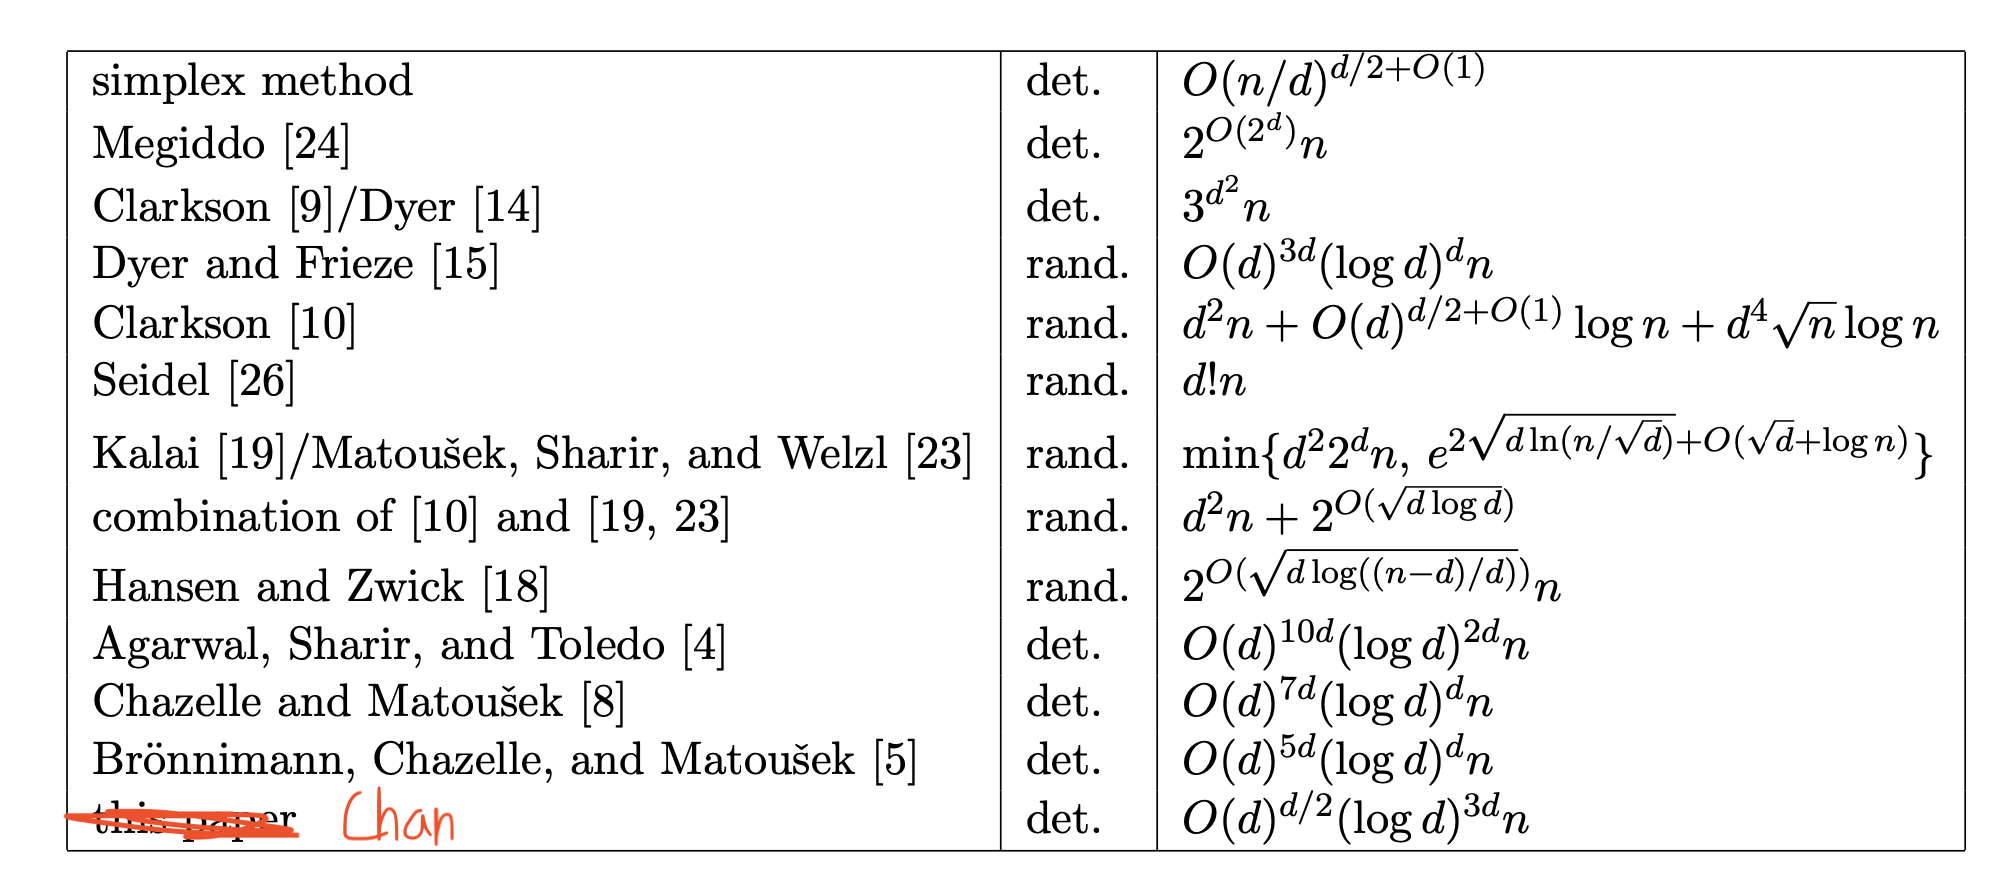
\includegraphics[width=\textwidth]{images/table.png}
        \caption{Algorithms for LP in low dimensions \footnote{table stolen from \url{https://dl.acm.org/doi/10.1145/3155312}}}
    \end{figure}
    \textbf{Can we use faster fixed dimension LP algorithms to get better complexity?}
\end{frame}

\begin{frame}[allowframebreaks]{LP-type problem}
    Algorithms for low dim LP are actually solving a more abstract problem.
    \begin{definition}[LP-type problem]
        Given a set $S$ and a function $f:S\to \R$. $f$ satisfies two properties:%
        \begin{itemize}
            \item Monotonicity: $\forall A\subseteq B\subseteq S, f(A)\leq f(B)\leq f(S)$.
            \item Locality: $\forall A\subseteq B\subseteq S$ and $\forall x\in S$, if $f(A) = f(B) = f(A \cup \{x\})$, then $f(A) = f(B \cup \{x\})$.
        \end{itemize}
    \end{definition}
    Linear programs(minimization) are LP-type problems.

    $B\subseteq S$ is a basis if $\forall B'\subsetneq B, f(B')<f(B)$. A set of `useful' constraints in a linear program is a basis.

    The combinatorial dimension is the size of the largest basis.

    If a LP problem has low dimension, then its combinatorial dimension is low. \textbf{What about the converse?}
    \newpage
    \begin{align*}
        \min &\sum_{i=1}^n f_i\\
        s.t. \quad f_i&\geq \alpha_j(a_i\cdot x -b_i)-\beta_j \quad \forall i\in[n], \forall j\\
        &\cdots
    \end{align*}%
    \textbf{Does our LP has low combinatorial dimension?}
    
    No. A basis contains at least $n$ constraints since otherwise some $f_i$ is unbounded.

    \begin{problem}
        Is it possible to formulate the pwl convex minimization problem as an LP-type problem with low combinatorial dimension?
    \end{problem}
\end{frame}



\begin{frame}{Aggregate the pwl convex functions}
    % blog posts
    The sum of pwl convex functions are still pwl convex. 
    \newline If we can compute $F=\sum f_i$ in $O(m)$ and the number of line segments on $F$ is also $O(m)$, then the corresponding LP will have low combinatorial dimension.
\end{frame}

\end{document}